\chapter{Discussion and Perspectives}
\label{ch:tool-eval}

In the previous chapter I described the goal and the set-up of each experiment, and reported their findings.
These findings allow us to evaluate different features of the Sensei plugin, as well as its use in the paved path methodology.
In this chapter I summarise the findings, explain the lessons we learned and how they can affect the development of Sensei in the future.

\summarybox{
Our findings and those of other research, show that customization of recipes can have a significant impact on the \gls{efp} rate, and hence the usability for the developer.
Using customized recipes results in a positive impact on the codebase since security issues are addressed truly as early as possible in the \gls{sdlc}.
If designed properly, applying the recipes regardless of context has minimal impact on performance, and helps improve code quality in many cases.

Security professionals report that creating these customized recipes with the recipe editor is easier than customizing rules of comparable tools.
Despite this, usability tests revealed that some features of the recipe editor can still be improved.
}


\section{Discussion}
\label{sec:eval-sensei}
\subsection{Installation and first use}
Because Sensei is distributed as an \gls{ide} plugin, it can be easily installed from the \gls{ide} itself, using features that many developers are familiar with.
None of the developers in any of the experiments needed more than several minutes to install the plugin.

After installation, the startup time of the \gls{ide} is not measurably affected by the tool.
Sensei only performs a license check, of which the duration is shorter than the measured variation in \gls{ide} start-up time.

In the early industry trial and the controlled experiment, customized Sensei rules were provided by us as a service.
In the usability tests and the most recent industry trial, the subjects were provided with public cookbooks that could be used as a starting point, but they were encouraged to create their own recipes.

In both groups we have observed developers who unknowingly addressed Sensei markings, thinking they were regular \gls{ide} markings.
This is strong evidence that the tool is intuitive and feels like a natural extension of the \gls{ide}.

\subsection{Recipes}
Sensei is a developer tool first, and this is evident from the recipes that are used in industry settings.
A significant portion of the recipes are related to the quality of the code rather than its security.
%Many Sensei recipes are also written to boost the productivity of the developer.
%One example is a set of recipes that was created to migrate from JUnit version 4 to version 5~\footnote{\url{https://junit.org/}}.

We have noticed, in practice, that security and quality are often closely related.
High quality code is easier to understand and maintain, and hence also to secure.
But often, writing high quality code can also lead to secure code in a more direct way.

Take the example of a \gls{sql} query.
Writing a data retrieval method of high quality means that the query is easy to understand, but also that the data is retrieved at high speed.
When the query is parameterized, the database can pre-compile a query plan, which speeds up the execution of the query.
Of course, using parameterized queries at the same time ensures that the query is safe from \gls{sql} injection.
Even if the current query did not use any (unsanitized) user input, using a parameterized query will protect it from future use.
It will also set a good example for future developers writing similar methods.
Developers will often copy existing code and make some changes to fit their needs.
After all, developers try to be as efficient as they can in delivering code.
If no parameterized queries are used, a subtle change can mean the difference between secure code or a vulnerability, as shown in Listings~\ref{lst:safe}~and~\ref{lst:unsafe}.

\begin{lstlisting}[float,language={Java},caption={This method concatenates an integer value to the query. An integer variable can not alter the query, and hence this method can not lead to SQL injection.},
float,label={lst:safe},abovecaptionskip=-0.0pt]
public ResultSet getUserById(int id){
    String query = "SELECT * FROM user WHERE id = " + id;
    PreparedStatement stmt = this.conn.prepareStatement(query);
    ResultSet rs = stmt.executeQuery();
    return rs;
}
\end{lstlisting}

\begin{lstlisting}[language={Java},caption={This method concatenates a String variable to the query. As a result it is vulnerable to SQL injection.}, float,label={lst:unsafe},abovecaptionskip=-0.0pt]
public ResultSet getUserById(String id){
    String query = "SELECT * FROM user WHERE id = " + id;
    PreparedStatement stmt = this.conn.prepareStatement(query);
    ResultSet rs = stmt.executeQuery();
    return rs;
}
\end{lstlisting}

In industry, recipes were created, both to help developers use libraries correctly, as well as to migrate to new libraries.
Security professionals reported that many wrapper libraries are used in their codebase to make the life of developers easier.
These wrapper libraries were rarely developed solely for security reasons, but often did include security automation.
It is clear that for such wrapper libraries, it is crucial that the recipes can easily be customized.

\subsection{Recipe editor}
When testing \gls{yaml} syntax and creating recipes from context, we observed a significant speed-up in writing recipes.
Even for users that were experienced with the old rule models, the preview panels in the new recipe editor and the context-aware suggestions greatly improve the recipe-writing process.

Security professionals report that Sensei is the easiest tool they have used when it comes to customizing recipes.
The majority of comparable tools allow writing custom rules or analyses in some way or another.
\todo[inline]{revisit after related work is finished}
Writing rules for these tools is done through complex, but well documented \glspl{api} (SpotBugs, Tricorder, Checkmarx) or more user-friendly custom formats such as \gls{xml} (Fortify, SecureAssist).
Of these, Checkmarx is the only one tool that provides a Query editor and manager, albeit not built into their static analysis tool.
For all other tools, the rule writers can use an \gls{ide} or text editor of their choice.
None of the tools allow creating rules on-the-fly in the code.
Sensei does allow this, which greatly improves the speed and usability of writing rules.
Related tools will be described in more detail in Chapter~\ref{ch:related}.

\subsubsection{Recipe features}
Because recipes can be created on-the-fly in the code, context-aware suggestions can be made, and testing of the recipes is more efficient since their markings can be observed live as the recipe is being created.
This live preview in the recipe editor is mentioned by the security professionals as Sensei's most useful feature.
Despite this, some of the features of the recipes and the recipe editor are not used as often or as effective as they could be.

When security professionals and developers create new recipes, they rarely use the code view.
In fact, we have noticed that the code view can be overwhelming for some users who want to avoid learning a new language.
To create recipes from scratch, and to adapt existing recipes, almost exclusively the \gls{ui} view is used.
The code view is only used by recipe-writers when copy-pasting recipes from the documentation or from recipes used as an example.
The \gls{gui} can be updated to better reflect this behaviour.
The \gls{ui} view should be the main focus when opening the recipe editor, and the code view can be made smaller as its main focus is to copy-paste examples.
The resulting \gls{gui} will have a similar user experience as the \gls{ui} provided by \gls{slack} to customize (and share) color themes, as shown in Figure~\ref{fig:slacktheme}.

\begin{figure}
  \centering
  %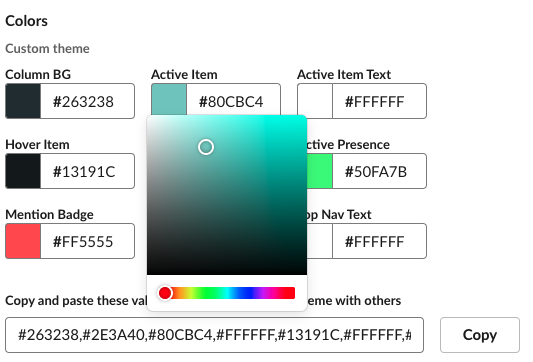
\includegraphics[width=0.75\textwidth]{slacktheme.png}
  \includegraphics[width=0.75\textwidth,page=16]{04-tools/figures/figures2.pdf}
  
  \caption[Slack theme editor]{The theme editor in slack provides an intuitive \gls{ui} interface on top to edit the theme, but also adds an code view and a copy button to allow fast and easy copy-pasting of existing themes.}
  \label{fig:slacktheme} 
\end{figure}

Security professionals report using the context-wizard to automatically generate recipes from context.
However, in usability tests, none of the tested users have used this features.
This indicates that the feature might not be clearly understood.
Instead of “create recipe for similar methodcalls”, it might be more effective to make the option in the menu adapt to the context, for example “create recipe for Runtime.exec methodcalls”.

Quick-fixes are added to nearly every recipe.
However, in some situations no fully functional quick-fix can be created and the developer is still required to make changes to the code after applying the quick-fix.
The template language that allows reusing parts of the original code is often required to create a working quick-fix.
However, the suggestion box in the quick-fix menu is not clearly visible to the users, and as a result these suggestions are rarely used.
The recipe-writer can still find them in the documentation or by copy pasting from other rules, but using this menu should be more convenient.
Currently, the variables are hidden by default and the ``Show variables" button is not prominent enough, as shown in Figure~\ref{fig:showvariables}.

\begin{figure}
  \centering
  %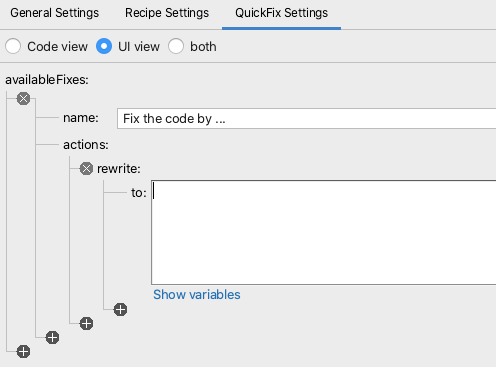
\includegraphics[width=0.75\textwidth]{showvariables.png}
  \includegraphics[width=0.75\textwidth,page=15]{04-tools/figures/figures2.pdf}
  \caption[Show variables button in the fix menu]{The suggestions in the quick-fix menu are hidden by default. Users do not make use of the ``Show variables" button that reveals them, as it does not attract their attention.}
  \label{fig:showvariables} 
\end{figure}

Scopes are used frequently in industry, almost exclusively to avoid creating \glspl{efp} and increase developer usability.
Most of the comparable tools operate in later stages of the \gls{sdlc}.
They perform scans during code review or testing phases.
Usability issues for these tools are less critical as they do not create markings that can disturb a developer during development.
Instead it is often a security expert who will analyze and prioritize the results of security scans by placing them into the bug tracking system.
Common features for those tools are integrations with common bug tracking systems to allow them to publish bugs automatically.

We observed that many tools provide functionality to disable certain rule reports through configuring security policies.
This is a necessary feature to remove or hide classic false positives.
However, this disabling of reports is designed to help security experts keep a good overview of the application state and to help prioritize more severe issues.
With the exception of the Fortify Security Assistant that disables rules to speed up the scans, disabling rules themselves is rarely supported with he goal to improve the usability of the developers.

\subsection{Feedback and remediation}
Sensei is distributed as an \gls{ide} plugin.
This allows it to reuse and extend existing \gls{ide} functionality, and naturally feel part of the existing tool kit of developers.
When interviewed, subjects of the usability tests reported that the markings and quick-fixes felt similar to those provided by the \gls{ide} itself.
They all indicated that they would use them frequently.

When analyzing newly written code, the longest time we have measured that is needed for the analyses to finish is 29 ms.
This is far below the threshold of 125 ms to be considered real time.
A developer is hence not hindered during development unless they are violating a coding guideline and need to use remediation.

When code is marked, the developer needs to spend some extra time understanding the issue and fixing it.
During the empirical experiment of Section~\ref{sec:experiment}, the mean observed remediation time of a guideline violation is 19 seconds.
On average, the use of Sensei increased the total development time with 11\%.
This is a relatively low increase considering the programming assignment was to complete security-critical features and hence the subjects were frequently confronted with feedback from the tool.
It is also important to note that for all of the subjects, the experiment was the first time they were making use of the tool.

During the experiment, 98.4\% of code markings shown by Sensei (n = 247) were resolved by the developers.
Out of the resolved code markings, 73.3\% were fixed using the quick-fixes.
All of the users (n = 15) used at least one quick-fix, with an average of 12.71 (s = 4.73) quick-fixes used.
The remaining code markings have been removed manually, either by fixing the violation or by removing the violating code entirely.
This is a high level of engagement, compared to the lower than 20\% ``Apply fix" rate reported by the code review tool Tricorder~\cite{sadowski2015tricorder}.
On average the subjects resolved the issue within 19.10 s (s = 25.22 s) of writing the violating \gls{api} call.
Developers appear to be spending comparatively little time understanding the issues and applying fixes.
By comparison, for Tricorder and SpotBugs the time between writing the violating code and fixing is usually several days~\cite{sadowski2015tricorder,ayewah2007using}.

In the experiment with Sensei, only 1.6\% of code markings were ignored, which is a low \gls{efp} rate.
After carefully improving their analyzers, Tricorder reached an \gls{efp} rate of around 5\%.
Despite its great attention to developer usability, during an experiment with ASIDE, only 63 of 101 markings were addressed~\cite{xie2011aside}.
When using SpotBugs, research reported that 58\% of the reported issues were never reviewed and out of the reviewed bugs, only 55\% were eventually fixed~\cite{ayewah2007using}.
We observe a big gap in \gls{efp} rates with Sensei and Tricorder having a rate of 5\% or lower on one hand, and Aside and SpotBugs having 38\% and 77\% on the other hand.
The reason for this might be the customization of rules.
Tricorder allows creating new analyzers and their quality is closely monitored.
For Sensei, developers are given carefully tailored rules, often written by the engineers themselves, and relevant to their project.
These efforts are clearly greatly improving the usability of the tool and hence the trust of the developers.

\subsubsection{Impact on security}
The usability measurements presented so far suggest that when Sensei is used, the secure coding guidelines are applied most of the time.
During the first undustry trial of the plugin, described in Section~\ref{sec:trial2018}, the client has tracked closely whether or not the enforced guidelines actually prevented the introduction of vulnerabilities early on.
The trial was done with five developers for the duration of three months.
They reported a total of over 200 confirmed bugs being prevented.
The most common issues involved sensitive information leakage and tapjacking vulnerabilities in their mobile application.

A limitation of the tool's local analyses is that they do not allow us to detect whether or not a certain input has already been sanitized before flowing into the routine being analyzed.
This is in line with our approach and goal of enforcing coding guidelines that defend every routine for future use, i.e., such that it is still secure whenever it might be reused with unsanitized data.
So if the local analyses identify a lack of local sanitization, the developer will be expected to let the routine sanitize that input again.
At first sight, this might result in the same data being sanitized multiple times within an application, which will negatively impact performance. 

In practice, however, this proves to be largely a non-issue.
In practice, \glspl{api} are not designed in a vacuum.
Instead they are developed with potential application architectures in mind.
Furthermore, when concrete applications are first designed, security and application architects also take into account best practices for secure architectures (that is, if they care for security-by-design).
Similarly, the coding guidelines can be co-designed with certain application architectures in mind.
Doing so provides an easy mitigation of the potential issue of redundant, multiple sanitizations.

For example, consider the case of \gls{xss} attacks.
It is a common misconception that in order to prevent stored \gls{xss} attacks, user input should be encoded before it is stored in the database.
A better recommendation is to encode the database output when it is used, as the stored data may be used in different contexts, requiring different encoding methods.
For example, a string value may be displayed on the \gls{html} page and also used in a JavaScript script on that same page, resulting in two different, but simultaneous escape requirements.
We learn that data should always be sanitized before it is stored in the database and encoded before it is displayed in the web or mobile application.
Since these are usually the ends of the data flow, no data needs to be sanitized or encoded twice.
If the rules are co-designed with the secure application architecture, it becomes trivial to enforce the sanitization and encoding routines at the correct locations in code. 
The above does not imply that Sensei is the one and only tool that solves all potential software development security issues.
To detect issues as early as possible, i.e., in real-time as the developer is writing code, analyses have to be light-weight.
This implies that all possible execution paths in the entire program cannot be exhaustively considered, and some types of vulnerabilities, including design flaws, can go undetected.
This is a common trade-off, therefore tools that are used early in the \gls{sdlc} such as Sensei should be complemented with more complete scanning solutions deployed later in the \gls{sdlc}.
\todo[inline]{revisit after related work}
Security professionals understand this.
In the second industry trial Sensei is complimented by five additional security tools: Fortify, Checkmarx, SonarQube, Semgrep, and FindBugs.

An example of this strategy also exists with multiple products of the same company. 
The Fortify Security Assistant \gls{ide} plugin is used earlier in the \gls{sdlc} than other Fortify tools, but only uses a subset of the available rules to improve developer usability.
It helps detect a set of vulnerabilities earlier, and hence saves money and time fixing those issues, but it does not provide the full protection that, e.g., Fortify on Demand does.
In the related work section, we will discuss where we consider Sensei to improve over Fortify Security Assistant as an early \gls{sdlc} tool.

\subsection{Project and team management}
\subsubsection{Compliance}
Coding guidelines can provide a good measure for security in a software product.
Where vulnerability scanning can only provide an indication of the vulnerability density, they do not provide the full picture.
In the case, for example, where a large number of \gls{sql} injections is found, this could indicate poor database security.
But it can also mean that there simply are a lot of database queries, with a large portion of them done securely.
For coding guidelines a relative measure can be designed, by comparing the number of guideline violations to the number of times the code complies to guidelines. Since complying to strong coding guidelines leads to secure code~\cite{banerjee2009software,tabassum2017comparing}, we get a better indication of the security in the software product.

While the plugin is useful as a tool to aid the developer, the option to measure guideline deployment also hints at its potential as a management tool.
Like we did for the empirical experiment, management can track the changes developers makes to projects and log the guideline violations that they introduce and fix, with or without aid of the quick-fixes.
Currently, this data is collected in the events databases on the machine of each developer.
In the future, these metrics will be collected and visualised on the \gls{scw} platform.
This makes the return on investment clear to companies using the tool.
Furthermore, this can be used to track the performance of individual developers, and then to give more targeted and individually tailored training.
This data can for example feed into the \gls{its} to improve its recommendations, as described in Section~\ref{sec:its-integration}.

\subsubsection{Integration in other stages of the \gls{sdlc}}
While individual performance can hence be measured and improved, with developers working in different branches, and hence different states of the project, it is hard to get a good overview that way.
To resolve this, we also give managers the possibility to use the plugin technology as a headless scan that can be performed from the command line.
However, in practice, we have noticed that the performance of this headless scan is lacking.
Especially for large codebases, memory usage becomes exceedingly large.
Security professionals also indicated that better integration with \gls{cicd} tools is needed.
This lack of automation in different stages of the \gls{sdlc} is critical for the security team.
The security professionals in the second industry trial have spent time and effort to recreate Sensei recipes in different tools in the \gls{sdlc} to compensate for Sensei's lack of \gls{cicd} integration.
While the tool is a developer tool first, it is also a security tool, and it is usually purchased by the security team.
Which is why it is important to show value for both user groups.

\subsubsection{Roll-out}
From experience, we learned that the plugin is ideally rolled out when new recipes do not mark any existing code.
This is when a project kicks off and zero lines of code have been written. 
Alternatively it can be rolled out when a new \gls{api} or library is introduced in the project and recipes will be written for this library or \gls{api}.
Few projects are developed from scratch, however, so the reality is that the plugin needs to work in an already developed product.
In that case, rolling the plugin out with all recipes switched on can be overwhelming to developers, as they are presented with a huge number of violations.
In addition, developers are often hesitant to fix issues they did not introduce in the code themselves, and they might not even have permission to change code that is not theirs.
This results in a large number of \glspl{efp}, which we want to avoid.

When developers create their own recipes from scratch, they are working on a certain branch of the project.
They usually create targeted recipes to fix or enforce small things in the project files they are working on.
When they create the recipe, they inspect the violations and fix the markings.
The recipe and fixed code are pushed to the codebase simultaneously.
This typically leads to few \glspl{efp}.
However, often the application security team of the company imposes recipes as well.
At one point, the security expert at a client of ours created a large number of recipes and imposed them onto the developers without fixing any of the resulting violations.
It did not come as a surprise that this resulted in a great number of \glspl{efp} and out of the 20 developers that had the tool installed, all of them had disabled its markings.
To avoid such failures, we recommend two approaches to keep the \gls{efp} rate low for imposed cookbooks.

Firstly, in the ideal scenario the security team creates a number of recipes and looks at their violations in the code to inspect their severity.
When recipes result in few violations, the team can safely roll out the recipes without resulting in too many \glspl{efp}.

The roll-out is more challenging when a recipe results in a large number of violations that are not trivially resolved.
In that case the security team should create a developer task force.
Their task is to create \glspl{api} to resolve the recipe hits.
They then turn the original recipe into a library adoption recipe and fix all marked code with this recipe.
In the process of doing so, many corner cases can be encountered that help to fine-tune both the \gls{api} and the recipe.
The new \gls{api}, the recipe, and all code fixes can be pushed to the codebase simultaneously. 

The ideal scenario might not apply in practice, however.
It is possible that the codebase is simply too large to start fixing all code markings.
We have had clients where a strong recipe resulted in over 3000 violations.
It can also be the case that when the security team creates a task force, this developer time is paid by the security budget, not the development budget.
In such cases it is not beneficial to spend developer time to fix the existing issues in the code before rolling out the recipe. 

We then instead recommend the second approach, in which the recipes are rolled out company-wide without fixing the code markings.
In order to keep the \gls{efp} rate sufficiently low, the violations are only shown partly.
For this purpose the option is added to the recipe editor, to only mark a recipe on newly developed code.
This way only new violations are shown (and resolved) without resulting in an overly large \gls{efp} rate.
\section{Perspectives}
\label{sec:sensei-perspectives}
%\todo[inline]{intro}

\subsection{Improved recipe creation}
\label{sec:improvedrulecreation}
Security professionals report that Sensei is the easiest tool they have used when it comes to creating new recipes.
They attribute this mostly to the preview panels in the recipe editor, rather than the specific \gls{yaml} syntax.
Developers, on the other hand, are not used to creating rules for any tools, so they usually have nothing to compare it to.
This is evident from the usability tests, where developers were more hesitant and more easily overwhelmed by the recipe editor compared to the security professionals.
To reduce this hesitation, in the previous section, a design was proposed that would make the \gls{ui} view the main focus in the recipe editor.
In this design the code view would only be used for copy-pasting recipes.
However, this still requires developers to create recipes for an analysis tool, a task they are not familiar with.

Instead, it might be possible to let developers create recipes simply by writing code.
Currently, Sensei is able to apply a code transformation based on instructions from a recipe.
In the future, it might be possible to do the opposite, and generate a Sensei recipe from a code transformation.
If this technology exists, the recipe editor can simply show two code panels side by side.
The left panel can be a static view of the current state of the code, while the right panel allows the developer to make (small) changes to the code.
A Sensei recipe can then be created from the code changes that can optionally be adjusted in the next step.

This technology would also enable automatic recipe creation methods, such as generating a recipe from a code patch in the code repository.
It might even be possible to dynamically suggest recipes while observing the developer during their normal workflow.
Previous research has been performed to identify \gls{api} rules for cryptography from code changes~\cite{paletov2018inferring}.
Efforts have also been made to automatically generate patches from code repositories and their histories, using different algorithms~\cite{weimer2009automatically}, including those learned from human-written patches~\cite{kim2013automatic} or correct code~\cite{long2016automatic}.
While this research tries to automatically patch bugs, the approaches can also be used to create recipes to apply the discovered patches more broadly and to do so during the writing of code rather than afterwards.
With some user interaction, such a tool might also be able to generate recipes (without fixes) from the output of traditional security tools.

This technology is part of ongoing research funded by a \gls{vlaio} \gls{oeno} project as of 2019.

\subsection{Adapting feedback to the skill level}
An important concept during the design and evaluation of the Sensei \gls{ide} plugin, is the \gls{efp} rate.
When many markings exist in the code that the developer does not intend to fix, i.e., when there is a high \gls{efp} rate, this might cause developers to be overwhelmed and ignore feedback from Sensei altogether.
To explain this concept, the example of \gls{os} command injection was used.
A simple and easy to understand recipe to avoid \gls{os} command injection, is to simply avoid all uses of \gls{os} commands.
A more experienced developer, however, will understand how \gls{os} commands can be used securely, for example to launch a different software application through a hard-coded command.
This recipe will lead to an \gls{efp} for an experienced developer, but might be more easily understood by a developer with no security skills than a more advanced recipe.

In other cases, recipes are created that detect (presumably) deliberate insecure configurations.
Take the example of cookies, where it is generally recommended to configure them as HttpOnly.
This prevents the cookies from being used in client-side scripts, and hence avoids some of the most common \gls{xss} attacks.
However, in some legitimate cases the developer might need to use a cookie in a client-side script, and to configure the cookie as such.
Of course, they have to take the security implication of this configuration into consideration.
For example, they will have to ensure that this is not used for security-sensitive cookies, such as session cookies.
A recipe that detects insecure configurations like this, will lead to \glspl{efp} for developers who need the features that are blocked by these configurations.

Both the example of the \gls{os} command and cookie configuration, lead to \glspl{efp} for security experts, but are still important recipes to enforce for a novice developer.
Fortunately, through integration with the \gls{scw} portal, a user ability estimate is available, such that the feedback for recipes like this can be adapted to the skill level of the developer.
For developers with a low ability level, this recipe can be shown as an error, while the more experienced developer can be shown a warning or information level marking.
The descriptions can also be adapted for each skill level.
The less experienced developer can be shown the simple and easy to understand guideline, to use the most secure configuration.
To a more skill full developer it will be less overwhelming to explain the security implications of the configuration, and how to mitigate them in other parts of the code.
Adapting \glspl{ui} is most often based on the experience of the user with the interface itself rather than their knowledge in a specific field~\cite{johnson2015bespoke, cockburn2014supporting}.
This research indicates that optimizing \gls{ui} design based on novice learning rather than long-term efficiency by experienced users can be counterproductive.
It remains future work to assess whether or not a more optimised \gls{ui} will be required for advanced Sensei users.